%!TEX program = xelatex
%# -*- coding: utf-8 -*-
%!TEX encoding = UTF-8 Unicode

\documentclass[12pt,oneside,a4paper]{article}\usepackage[]{graphicx}\usepackage[]{xcolor}
%% maxwidth is the original width if it is less than linewidth
%% otherwise use linewidth (to make sure the graphics do not exceed the margin)
\makeatletter
\def\maxwidth{ %
  \ifdim\Gin@nat@width>\linewidth
    \linewidth
  \else
    \Gin@nat@width
  \fi
}
\makeatother

\definecolor{fgcolor}{rgb}{0, 0, 0}
\newcommand{\hlnum}[1]{\textcolor[rgb]{0,0,0}{#1}}%
\newcommand{\hlstr}[1]{\textcolor[rgb]{0,0,1}{#1}}%
\newcommand{\hlcom}[1]{\textcolor[rgb]{0.443,0.478,0.702}{#1}}%
\newcommand{\hlopt}[1]{\textcolor[rgb]{0,0,0}{#1}}%
\newcommand{\hlstd}[1]{\textcolor[rgb]{0,0,0}{#1}}%
\newcommand{\hlkwa}[1]{\textcolor[rgb]{0.498,0,0.333}{\textbf{#1}}}%
\newcommand{\hlkwb}[1]{\textcolor[rgb]{0.498,0,0.333}{\textbf{#1}}}%
\newcommand{\hlkwc}[1]{\textcolor[rgb]{0.498,0,0.333}{\textbf{#1}}}%
\newcommand{\hlkwd}[1]{\textcolor[rgb]{0,0,0}{#1}}%

\usepackage{framed}
\makeatletter
\newenvironment{kframe}{%
 \def\at@end@of@kframe{}%
 \ifinner\ifhmode%
  \def\at@end@of@kframe{\end{minipage}}%
  \begin{minipage}{\columnwidth}%
 \fi\fi%
 \def\FrameCommand##1{\hskip\@totalleftmargin \hskip-\fboxsep
 \colorbox{shadecolor}{##1}\hskip-\fboxsep
     % There is no \\@totalrightmargin, so:
     \hskip-\linewidth \hskip-\@totalleftmargin \hskip\columnwidth}%
 \MakeFramed {\advance\hsize-\width
   \@totalleftmargin\z@ \linewidth\hsize
   \@setminipage}}%
 {\par\unskip\endMakeFramed%
 \at@end@of@kframe}
\makeatother

\definecolor{shadecolor}{rgb}{.97, .97, .97}
\definecolor{messagecolor}{rgb}{0, 0, 0}
\definecolor{warningcolor}{rgb}{1, 0, 1}
\definecolor{errorcolor}{rgb}{1, 0, 0}
\newenvironment{knitrout}{}{} % an empty environment to be redefined in TeX

\usepackage{alltt}
\usepackage{geometry}
\geometry{verbose,tmargin=2cm,bmargin=2cm,lmargin=2cm,rmargin=2cm}
\usepackage[pdfusetitle,
 bookmarks=true,bookmarksnumbered=true,bookmarksopen=true,bookmarksopenlevel=2,
 breaklinks=false,pdfborder={0 0 1},backref=false,colorlinks=false]
 {hyperref}
\hypersetup{pdfstartview={XYZ null null 1}}
\usepackage{url}
\setcounter{secnumdepth}{2}
\setcounter{tocdepth}{2}
\usepackage{microtype}

\usepackage{amsmath, amsthm, amssymb, amsfonts}

\usepackage{algorithm}
\usepackage{algorithmic}
\renewcommand{\algorithmicrequire}{\textbf{Input:}} 
\renewcommand{\algorithmicensure}{\textbf{Output:}} 

\usepackage[sc]{mathpazo}
\linespread{1.1}
\usepackage[T1]{fontenc}


\usepackage{graphics}
\usepackage{graphicx}
\usepackage[figure]{hypcap}
\usepackage[hypcap]{caption}
\usepackage{tikz}
%\usepackage{grffile} 
%\usepackage{float} 
\usepackage{pdfpages}

\usepackage{multirow}
\usepackage{booktabs}
\usepackage{threeparttable}

%\usepackage[square,numbers,super,comma,sort]{natbib}
%\usepackage[backend=biber, style=nature, sorting=none, isbn=false, url=false, doi=false]{biblatex}
%\addbibresource{ref.bib}
%\usepackage[]{authblk}

\usepackage{verbatim}

\newcommand{\problem}[1]
{
    \clearpage
    \section*{Problem {#1}}
}

\newcommand{\subproblem}[1]
{
    \subsection*{Problem {#1}}
}


\newcommand{\solution}
{
    \vspace{15pt}
    \noindent\ignorespaces\textbf{\large Solution}
}

\usepackage{fancyhdr}
\usepackage{extramarks}
\lhead{\hmwkAuthorName}
\chead{\hmwkTitle}
\rhead{\firstxmark}
\cfoot{\thepage}

\newcommand{\hmwkTitle}{STAT 8051 HW 2}
\newcommand{\hmwkAuthorName}{Jingxiang Li}

\setlength\headheight{15pt}
\setlength\parindent{0pt}
\setlength{\parskip}{0.5em}

\newcommand{\m}[1]{\texttt{{#1}}}


\pagestyle{fancy}

\title{\hmwkTitle}
\author{\hmwkAuthorName}
\date{\today}
\IfFileExists{upquote.sty}{\usepackage{upquote}}{}
\begin{document}

\maketitle



\problem{3.2}
\textbf{Added-variable plots} (Data file: \texttt{UN11}) This problem uses the United Nations example in Section 3.1 to demonstrate many of the properties of added-variable plots. This problem is based on the mean function \texttt{fertility $\sim$ log(ppgdp) + pctUrban}. There is nothing special about a two-predictor regression mean function, but we are using this case for simplicity.

\subproblem{3.2.1}
Examine the scatterplot matrix for (\texttt{fertility, log(ppgdp), pctUrban}), and comment on the marginal relationships.

\solution
\begin{knitrout}
\definecolor{shadecolor}{rgb}{1, 1, 1}\color{fgcolor}\begin{kframe}
\begin{alltt}
\hlkwd{require}\hlstd{(}\hlkwc{package} \hlstd{=} \hlstr{"alr4"}\hlstd{)}

\hlstd{data} \hlkwb{<-} \hlkwd{data.frame}\hlstd{(UN11}\hlopt{$}\hlstd{fertility,} \hlkwd{log}\hlstd{(UN11}\hlopt{$}\hlstd{ppgdp), UN11}\hlopt{$}\hlstd{pctUrban)}
\hlstd{panel.cor} \hlkwb{<-} \hlkwa{function}\hlstd{(}\hlkwc{x}\hlstd{,} \hlkwc{y}\hlstd{,} \hlkwc{digits} \hlstd{=} \hlnum{2}\hlstd{,} \hlkwc{prefix} \hlstd{=} \hlstr{"cor = "}\hlstd{,} \hlkwc{cex.cor}\hlstd{,} \hlkwc{...}\hlstd{)}
\hlstd{\{}
    \hlstd{usr} \hlkwb{<-} \hlkwd{par}\hlstd{(}\hlstr{"usr"}\hlstd{);} \hlkwd{on.exit}\hlstd{(}\hlkwd{par}\hlstd{(usr))}
    \hlkwd{par}\hlstd{(}\hlkwc{usr} \hlstd{=} \hlkwd{c}\hlstd{(}\hlnum{0}\hlstd{,} \hlnum{1}\hlstd{,} \hlnum{0}\hlstd{,} \hlnum{1}\hlstd{))}
    \hlstd{r} \hlkwb{<-} \hlkwd{abs}\hlstd{(}\hlkwd{cor}\hlstd{(x, y))}
    \hlstd{txt} \hlkwb{<-} \hlkwd{format}\hlstd{(}\hlkwd{c}\hlstd{(r,} \hlnum{0.123456789}\hlstd{),} \hlkwc{digits} \hlstd{= digits)[}\hlnum{1}\hlstd{]}
    \hlstd{txt} \hlkwb{<-} \hlkwd{paste0}\hlstd{(prefix, txt)}
    \hlkwa{if}\hlstd{(}\hlkwd{missing}\hlstd{(cex.cor)) cex.cor} \hlkwb{<-} \hlnum{0.8}\hlopt{/}\hlkwd{strwidth}\hlstd{(txt)}
    \hlkwd{text}\hlstd{(}\hlnum{0.5}\hlstd{,} \hlnum{0.5}\hlstd{, txt,} \hlkwc{cex} \hlstd{= cex.cor} \hlopt{*} \hlstd{r)}
\hlstd{\}}

\hlkwd{pairs}\hlstd{(data,} \hlkwc{lower.panel} \hlstd{= panel.smooth,} \hlkwc{upper.panel} \hlstd{= panel.cor)}
\end{alltt}
\end{kframe}

{\centering 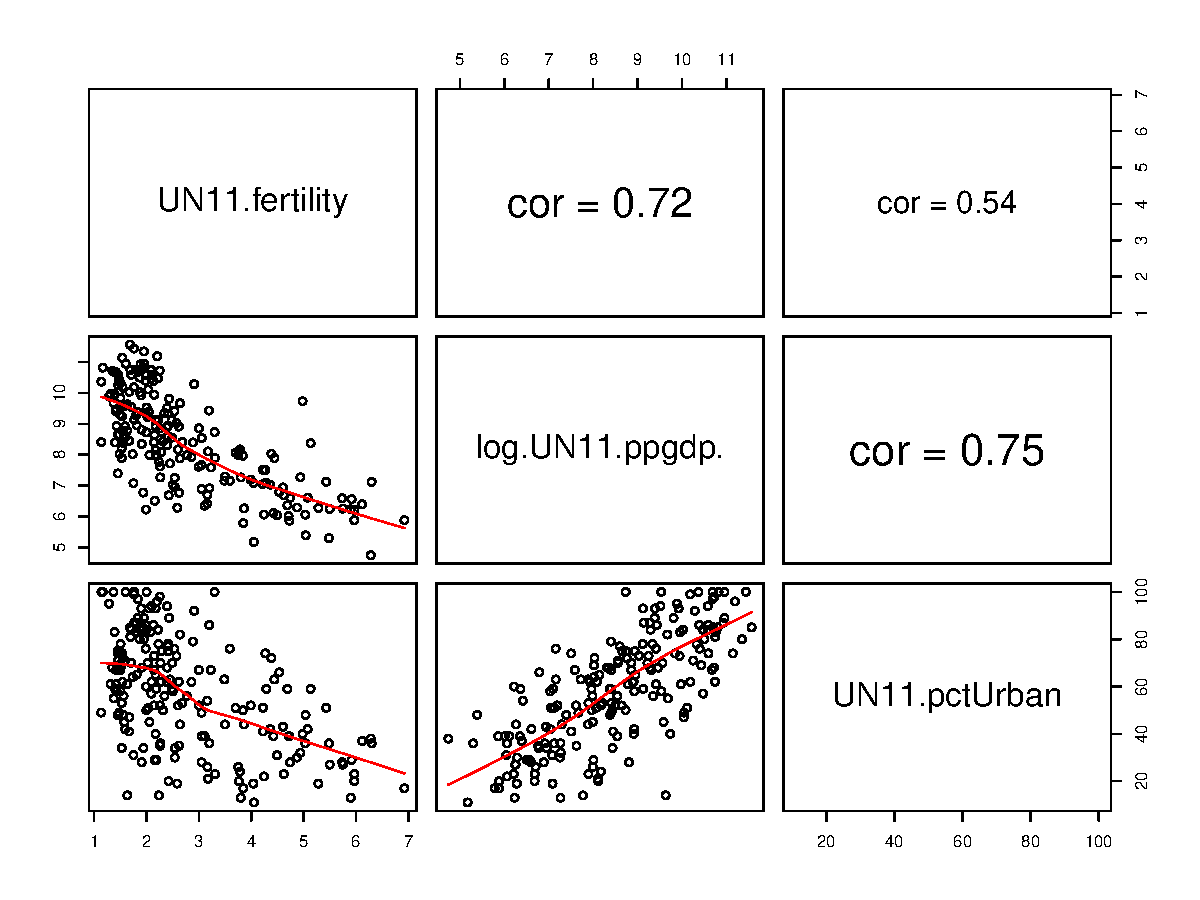
\includegraphics[width=.9\linewidth]{figure/p321} 

}



\end{knitrout}

This is the Scatterplot Matrix for (\texttt{fertility, log(ppgdp), pctUrban}). First, this graph shows decreasing tendencies of the response over two predictors respectively, suggesting that linear regression of \texttt{fertility} over these two predictors dose make sense. Plus, the correlation coefficients between response and two predictors also illustrate that there exists linear relationship among these variables. However, the bad news is that this graph also illustrates strong collinearity between two predictors, which means that the regression model we are going to establish may not give valid results about any individual predictor.

\subproblem{3.2.2}
Fit the two simple regressions for \m{fertility $\sim$ log(ppgdp)} and for \m{fertility $\sim$ pctUrban}, and verify that the slope coefficients are significantly different from 0 at any conventional level of significance.

\solution
\begin{knitrout}
\definecolor{shadecolor}{rgb}{1, 1, 1}\color{fgcolor}\begin{kframe}
\begin{alltt}
\hlstd{m1} \hlkwb{<-} \hlkwd{lm}\hlstd{(fertility} \hlopt{~} \hlkwd{log}\hlstd{(ppgdp),} \hlkwc{data} \hlstd{= UN11)}
\hlstd{m2} \hlkwb{<-} \hlkwd{lm}\hlstd{(fertility} \hlopt{~} \hlstd{pctUrban,} \hlkwc{data} \hlstd{= UN11)}
\hlkwd{summary}\hlstd{(m1)}
\end{alltt}
\begin{verbatim}
## 
## Call:
## lm(formula = fertility ~ log(ppgdp), data = UN11)
## 
## Residuals:
##     Min      1Q  Median      3Q     Max 
## -2.1631 -0.6451 -0.0659  0.6248  3.0052 
## 
## Coefficients:
##             Estimate Std. Error t value Pr(>|t|)    
## (Intercept)   8.0097     0.3653    21.9   <2e-16 ***
## log(ppgdp)   -0.6201     0.0424   -14.6   <2e-16 ***
## ---
## Signif. codes:  0 '***' 0.001 '**' 0.01 '*' 0.05 '.' 0.1 ' ' 1
## 
## Residual standard error: 0.93 on 197 degrees of freedom
## Multiple R-squared:  0.52,	Adjusted R-squared:  0.518 
## F-statistic:  213 on 1 and 197 DF,  p-value: <2e-16
\end{verbatim}
\begin{alltt}
\hlkwd{summary}\hlstd{(m2)}
\end{alltt}
\begin{verbatim}
## 
## Call:
## lm(formula = fertility ~ pctUrban, data = UN11)
## 
## Residuals:
##    Min     1Q Median     3Q    Max 
## -2.493 -0.779 -0.147  0.652  2.903 
## 
## Coefficients:
##             Estimate Std. Error t value Pr(>|t|)    
## (Intercept)  4.55982    0.21368   21.34   <2e-16 ***
## pctUrban    -0.03105    0.00342   -9.08   <2e-16 ***
## ---
## Signif. codes:  0 '***' 0.001 '**' 0.01 '*' 0.05 '.' 0.1 ' ' 1
## 
## Residual standard error: 1.13 on 197 degrees of freedom
## Multiple R-squared:  0.295,	Adjusted R-squared:  0.291 
## F-statistic: 82.4 on 1 and 197 DF,  p-value: <2e-16
\end{verbatim}
\end{kframe}
\end{knitrout}

m1 is the simple regression model for \m{fertility $\sim$ log(ppgdp)}, m2 is for \m{fertility $\sim$ pctUrban}. To see whether the slope coefficients are zero, we only need refer to the p-values of F-test given by two models. Note that the p-values given by two models are all $<2e-16$, suggesting that both two slope coefficients are significantly different from 0, at any conventional level of significance.

\subproblem{3.2.3}
Obtain the added-variable plots for both predictors. Based on the added-variable plots, is \m{log(ppgdp)} useful after adjusting for \m{pctUrban}, and similarly, is \m{pctUrban }useful after adjusting for \m{log(ppgdp)}? Compute the estimated mean function with both predictors included as regressors, and verify the findings of the added-variable plots.

\solution
\begin{knitrout}
\definecolor{shadecolor}{rgb}{1, 1, 1}\color{fgcolor}\begin{kframe}
\begin{alltt}
\hlkwd{require}\hlstd{(}\hlkwc{package} \hlstd{=} \hlstr{"ggplot2"}\hlstd{)}
\hlkwd{require}\hlstd{(}\hlkwc{package} \hlstd{=} \hlstr{"gridExtra"}\hlstd{)}

\hlstd{e_f2lp} \hlkwb{<-} \hlstd{m1}\hlopt{$}\hlstd{residuals}
\hlstd{e_f2pU} \hlkwb{<-} \hlstd{m2}\hlopt{$}\hlstd{residuals}
\hlstd{e_lp2pU} \hlkwb{<-} \hlkwd{lm}\hlstd{(}\hlkwd{log}\hlstd{(ppgdp)} \hlopt{~} \hlstd{pctUrban,} \hlkwc{data} \hlstd{= UN11)}\hlopt{$}\hlstd{residuals}
\hlstd{e_pU2lp} \hlkwb{<-} \hlkwd{lm}\hlstd{(pctUrban} \hlopt{~} \hlkwd{log}\hlstd{(ppgdp),} \hlkwc{data} \hlstd{= UN11)}\hlopt{$}\hlstd{residuals}

\hlstd{p1} \hlkwb{<-} \hlkwd{ggplot}\hlstd{(}\hlkwd{data.frame}\hlstd{(}\hlkwc{x} \hlstd{= e_pU2lp,} \hlkwc{y} \hlstd{= e_f2lp),} \hlkwd{aes}\hlstd{(}\hlkwc{x} \hlstd{= x,} \hlkwc{y} \hlstd{= y))}
\hlstd{p1} \hlkwb{<-} \hlstd{p1} \hlopt{+} \hlkwd{geom_point}\hlstd{()}
\hlstd{p1} \hlkwb{<-} \hlstd{p1} \hlopt{+} \hlkwd{geom_smooth}\hlstd{(}\hlkwc{formula} \hlstd{= y} \hlopt{~} \hlstd{x,} \hlkwc{method} \hlstd{=} \hlstr{"lm"}\hlstd{,} \hlkwc{se} \hlstd{=} \hlnum{FALSE}\hlstd{)}
\hlstd{p1} \hlkwb{<-} \hlstd{p1} \hlopt{+} \hlkwd{theme_bw}\hlstd{()} \hlopt{+} \hlkwd{theme}\hlstd{(}\hlkwc{text} \hlstd{=} \hlkwd{element_text}\hlstd{(}\hlkwc{size} \hlstd{=} \hlnum{14}\hlstd{))}
\hlstd{p1} \hlkwb{<-} \hlstd{p1} \hlopt{+} \hlkwd{ggtitle}\hlstd{(}\hlstr{"pctUrban after log(ppgdp)"}\hlstd{)}

\hlstd{p2} \hlkwb{<-} \hlkwd{ggplot}\hlstd{(}\hlkwd{data.frame}\hlstd{(}\hlkwc{x} \hlstd{= e_lp2pU,} \hlkwc{y} \hlstd{= e_f2pU),} \hlkwd{aes}\hlstd{(}\hlkwc{x} \hlstd{= x,} \hlkwc{y} \hlstd{= y))}
\hlstd{p2} \hlkwb{<-} \hlstd{p2} \hlopt{+} \hlkwd{geom_point}\hlstd{()}
\hlstd{p2} \hlkwb{<-} \hlstd{p2} \hlopt{+} \hlkwd{geom_smooth}\hlstd{(}\hlkwc{formula} \hlstd{= y} \hlopt{~} \hlstd{x,} \hlkwc{method} \hlstd{=} \hlstr{"lm"}\hlstd{,} \hlkwc{se} \hlstd{=} \hlnum{FALSE}\hlstd{)}
\hlstd{p2} \hlkwb{<-} \hlstd{p2} \hlopt{+} \hlkwd{theme_bw}\hlstd{()} \hlopt{+} \hlkwd{theme}\hlstd{(}\hlkwc{text} \hlstd{=} \hlkwd{element_text}\hlstd{(}\hlkwc{size} \hlstd{=} \hlnum{14}\hlstd{))}
\hlstd{p2} \hlkwb{<-} \hlstd{p2} \hlopt{+} \hlkwd{ggtitle}\hlstd{(}\hlstr{"log(ppgdp) after pctUrban"}\hlstd{)}
\hlkwd{grid.arrange}\hlstd{(p1, p2,} \hlkwc{ncol}\hlstd{=}\hlnum{2}\hlstd{)}
\end{alltt}
\end{kframe}

{\centering 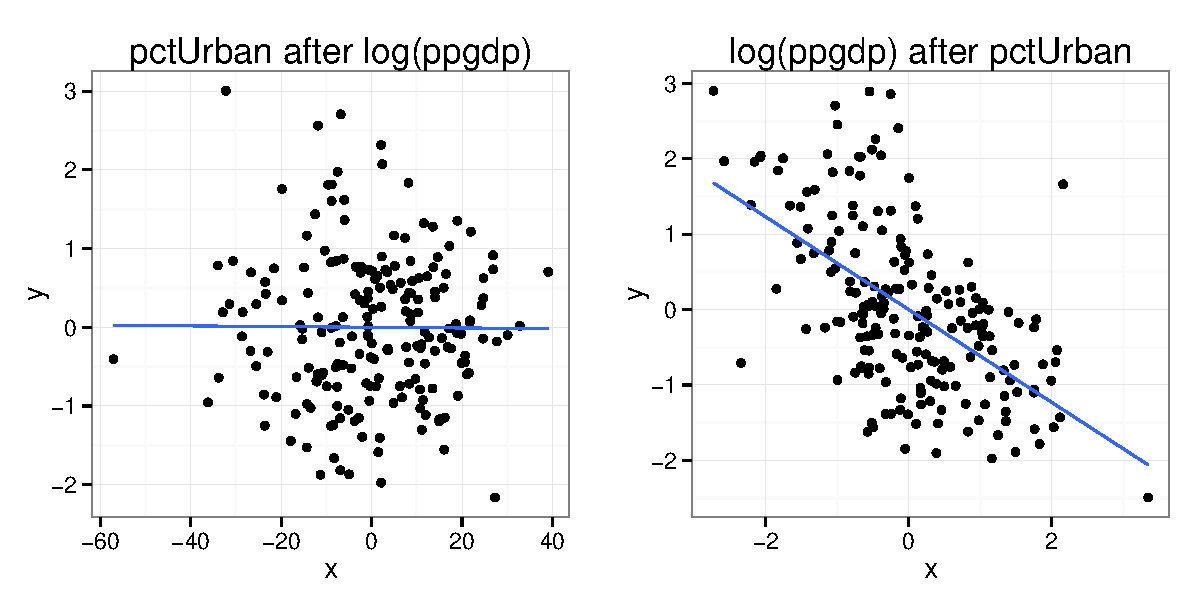
\includegraphics[width=.9\linewidth]{figure/p323} 

}



\end{knitrout}

Graph on the left side is the added-variable plot for \m{pctUrban} after \m{log(ppgdp)}, similarly, the one on the right side is the plot for \m{log(ppgdp)} after \m{pctUrban}. From these two graphs we see that \m{log(ppgdp)} is still useful to explain the variance of response after adjusting for \m{pctUrban}. However, it seems that after adjusting for \m{log(ppgdp)}, \m{pctUrban} loses its power of explaining the response term, suggesting that the coefficient of \m{pctUrban} in the two predictor regression model should be insignificant. Let's see.

\begin{knitrout}
\definecolor{shadecolor}{rgb}{1, 1, 1}\color{fgcolor}\begin{kframe}
\begin{alltt}
\hlkwd{summary}\hlstd{(}\hlkwd{lm}\hlstd{(fertility} \hlopt{~} \hlkwd{log}\hlstd{(ppgdp)} \hlopt{+} \hlstd{pctUrban,} \hlkwc{data} \hlstd{= UN11))}
\end{alltt}
\begin{verbatim}
## 
## Call:
## lm(formula = fertility ~ log(ppgdp) + pctUrban, data = UN11)
## 
## Residuals:
##    Min     1Q Median     3Q    Max 
## -2.151 -0.649 -0.066  0.632  2.991 
## 
## Coefficients:
##              Estimate Std. Error t value Pr(>|t|)    
## (Intercept)  7.993270   0.399337   20.02   <2e-16 ***
## log(ppgdp)  -0.615142   0.064156   -9.59   <2e-16 ***
## pctUrban    -0.000439   0.004266   -0.10     0.92    
## ---
## Signif. codes:  0 '***' 0.001 '**' 0.01 '*' 0.05 '.' 0.1 ' ' 1
## 
## Residual standard error: 0.933 on 196 degrees of freedom
## Multiple R-squared:  0.52,	Adjusted R-squared:  0.515 
## F-statistic:  106 on 2 and 196 DF,  p-value: <2e-16
\end{verbatim}
\end{kframe}
\end{knitrout}

Note that in this two predictor regression model, as what we expected, the p-value of \m{log(ppgdp)} is negligible, which means \m{log(ppgdp)} is significant in this model. On the other side, the p-value of \m{pctUrban} is $0.918$! which strongly suggests that \m{pctUrban} is not significant in this two predictor model.

\subproblem{3.2.4}
Show that the estimated coefficient for \m{log(ppgdp)} is the same as the estimated slope in the added-variable plot for \m{log(ppgdp)} after \m{pctUrban}. This correctly suggests that all the estimates in a multiple linear regression model are adjusted for all the other regressors in the mean function.

\solution
\begin{knitrout}
\definecolor{shadecolor}{rgb}{1, 1, 1}\color{fgcolor}\begin{kframe}
\begin{alltt}
\hlstd{m1} \hlkwb{<-} \hlkwd{coef}\hlstd{(}\hlkwd{lm}\hlstd{(fertility} \hlopt{~} \hlkwd{log}\hlstd{(ppgdp)} \hlopt{+} \hlstd{pctUrban,} \hlkwc{data} \hlstd{= UN11))}
\hlstd{m2} \hlkwb{<-} \hlkwd{coef}\hlstd{(}\hlkwd{lm}\hlstd{(e_f2pU} \hlopt{~} \hlstd{e_lp2pU))}
\hlstd{m1}
\end{alltt}
\begin{verbatim}
## (Intercept)  log(ppgdp)    pctUrban 
##   7.9932699  -0.6151425  -0.0004393
\end{verbatim}
\begin{alltt}
\hlstd{m2}
\end{alltt}
\begin{verbatim}
## (Intercept)     e_lp2pU 
##  -1.162e-16  -6.151e-01
\end{verbatim}
\end{kframe}
\end{knitrout}

In the code chunk above, \m{m1} is the two predictor model and \m{m2} the added-variable model for \m{log(ppgdp)} after \m{pctUrban}. We see that the coefficient value of \m{log(ppgdp)} in two predictor model is the same as the slope coefficient in the added-variable model, suggesting that all the estimates in a multiple linear regression model are adjusted for all the other regressors in the mean function.

\subproblem{3.2.5}
Show that the residuals in the added-variable plot are identical to the residuals from the mean function with both predictors.

\solution
\begin{knitrout}
\definecolor{shadecolor}{rgb}{1, 1, 1}\color{fgcolor}\begin{kframe}
\begin{alltt}
\hlstd{m1} \hlkwb{<-} \hlkwd{lm}\hlstd{(fertility} \hlopt{~} \hlkwd{log}\hlstd{(ppgdp)} \hlopt{+} \hlstd{pctUrban,} \hlkwc{data} \hlstd{= UN11)}
\hlstd{m2} \hlkwb{<-} \hlkwd{lm}\hlstd{(e_f2pU} \hlopt{~} \hlstd{e_lp2pU)}
\hlstd{p} \hlkwb{<-} \hlkwd{ggplot}\hlstd{(}\hlkwd{data.frame}\hlstd{(m1}\hlopt{$}\hlstd{residuals, m2}\hlopt{$}\hlstd{residuals),}
            \hlkwd{aes}\hlstd{(}\hlkwc{x} \hlstd{= m1}\hlopt{$}\hlstd{residuals,} \hlkwc{y} \hlstd{= m2}\hlopt{$}\hlstd{residuals))}
\hlstd{p} \hlkwb{<-} \hlstd{p} \hlopt{+} \hlkwd{geom_point}\hlstd{()}
\hlstd{p} \hlkwb{<-} \hlstd{p} \hlopt{+} \hlkwd{theme_bw}\hlstd{()} \hlopt{+} \hlkwd{theme}\hlstd{(}\hlkwc{text} \hlstd{=} \hlkwd{element_text}\hlstd{(}\hlkwc{size} \hlstd{=} \hlnum{12}\hlstd{))}
\hlstd{p} \hlkwb{<-} \hlstd{p} \hlopt{+} \hlkwd{ggtitle}\hlstd{(}\hlstr{"Residuals VS Residuals"}\hlstd{)}
\hlstd{p} \hlkwb{<-} \hlstd{p} \hlopt{+} \hlkwd{xlab}\hlstd{(}\hlstr{"Residuals from added-variable model"}\hlstd{)} \hlopt{+}
    \hlkwd{ylab}\hlstd{(}\hlstr{"Residuals from two predictor model"}\hlstd{)}
\hlstd{p}
\end{alltt}
\end{kframe}

{\centering 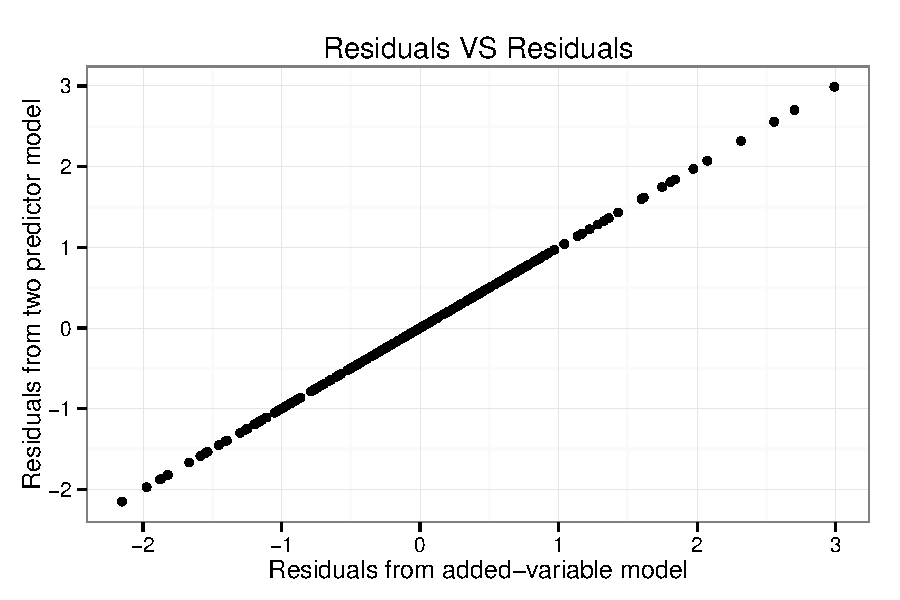
\includegraphics[width=.8\linewidth]{figure/p325} 

}



\end{knitrout}

This graph is means to show that residuals from two models are the same. the x axis is the "residuals from added-variable model", the y axis is the "residuals from two predictor model". It shows that all points, representing residual pairs from two models for each case in this data set, are precisely on the line $y = x$, suggesting that the residuals in the added-variable plot are identical to the residuals from the mean function with both predictors. 

\subproblem{3.2.6}
Show that the t-test for the coefficient for \m{log(ppgdp)} is not quite the same from the added-variable plot and from the regression with both regressors, and explain why they are slightly different.

\solution
\begin{knitrout}
\definecolor{shadecolor}{rgb}{1, 1, 1}\color{fgcolor}\begin{kframe}
\begin{alltt}
\hlkwd{summary}\hlstd{(m1)}
\end{alltt}
\begin{verbatim}
## 
## Call:
## lm(formula = fertility ~ log(ppgdp) + pctUrban, data = UN11)
## 
## Residuals:
##    Min     1Q Median     3Q    Max 
## -2.151 -0.649 -0.066  0.632  2.991 
## 
## Coefficients:
##              Estimate Std. Error t value Pr(>|t|)    
## (Intercept)  7.993270   0.399337   20.02   <2e-16 ***
## log(ppgdp)  -0.615142   0.064156   -9.59   <2e-16 ***
## pctUrban    -0.000439   0.004266   -0.10     0.92    
## ---
## Signif. codes:  0 '***' 0.001 '**' 0.01 '*' 0.05 '.' 0.1 ' ' 1
## 
## Residual standard error: 0.933 on 196 degrees of freedom
## Multiple R-squared:  0.52,	Adjusted R-squared:  0.515 
## F-statistic:  106 on 2 and 196 DF,  p-value: <2e-16
\end{verbatim}
\begin{alltt}
\hlkwd{summary}\hlstd{(m2)}
\end{alltt}
\begin{verbatim}
## 
## Call:
## lm(formula = e_f2pU ~ e_lp2pU)
## 
## Residuals:
##    Min     1Q Median     3Q    Max 
## -2.151 -0.649 -0.066  0.632  2.991 
## 
## Coefficients:
##              Estimate Std. Error t value Pr(>|t|)    
## (Intercept) -1.16e-16   6.60e-02    0.00        1    
## e_lp2pU     -6.15e-01   6.40e-02   -9.61   <2e-16 ***
## ---
## Signif. codes:  0 '***' 0.001 '**' 0.01 '*' 0.05 '.' 0.1 ' ' 1
## 
## Residual standard error: 0.93 on 197 degrees of freedom
## Multiple R-squared:  0.319,	Adjusted R-squared:  0.316 
## F-statistic: 92.4 on 1 and 197 DF,  p-value: <2e-16
\end{verbatim}
\end{kframe}
\end{knitrout}

In the code chunk above, \m{m1} is the two predictor model and \m{m2} the added-variable model for \m{log(ppgdp)} after \m{pctUrban}. It's easy to see that two t-values are different, suggesting that the t-test for the coefficient for \m{log(ppgdp)} is not quite the same from the added-variable plot and from the regression with both regressors. But it's only a matter of degree of freedom. In \m{m1}, the degree of freedom is $n - 3$, but in \m{m2}, the degree of freedom is $n - 2$. In fact, after adjusting the degree of freedom, the t-test of these two models are essentially the same. 

\problem{4.2}
(Data file: \m{Transact}) The data in this example consists of a sample of branches of a large Australian bank (Cunningham and Heathcote, 1989). Each branch makes transactions of two types, and for each of the branches we have recorded the number \m{t1} of type 1 transactions and the number \m{t2} of type 2 transactions. The response is \m{time}, the total minutes of labor used by the branch. Define $a = (\m{t2} + \m{t1})/2$ to be the average transaction time, and $d = \m{t1} - \m{t2}$, and fit the following four mean functions
$$\begin{array}{lll}
    M1: E(time |t1, t2 ) &=& \beta_{0,1} + \beta_{1,1}t1 + \beta_{2,1}t2\\
    M2: E(time |t1, t2 ) &=& \beta_{0,2} + \beta_{3,2}a + \beta_{4,2}d\\
    M3: E(time |t1, t2 ) &=& \beta_{0,3} + \beta_{2,3}t2 + \beta_{4,3}d\\
    M4: E(time |t1, t2 ) &=& \beta_{0,4} + \beta_{1,4}t1 + \beta_{2,4}t2 + \beta_{3,4}a + \beta_{4,4}d
\end{array}$$

\solution
\begin{knitrout}
\definecolor{shadecolor}{rgb}{1, 1, 1}\color{fgcolor}\begin{kframe}
\begin{alltt}
\hlstd{Transact}\hlopt{$}\hlstd{a} \hlkwb{<-} \hlstd{(Transact}\hlopt{$}\hlstd{t1} \hlopt{+} \hlstd{Transact}\hlopt{$}\hlstd{t2)} \hlopt{/} \hlnum{2}
\hlstd{Transact}\hlopt{$}\hlstd{d} \hlkwb{<-} \hlstd{(Transact}\hlopt{$}\hlstd{t1} \hlopt{-} \hlstd{Transact}\hlopt{$}\hlstd{t2)}
\hlstd{m1} \hlkwb{<-} \hlkwd{lm}\hlstd{(time} \hlopt{~} \hlstd{t1} \hlopt{+} \hlstd{t2,} \hlkwc{data} \hlstd{= Transact)}
\hlstd{m2} \hlkwb{<-} \hlkwd{lm}\hlstd{(time} \hlopt{~} \hlstd{a} \hlopt{+} \hlstd{d,} \hlkwc{data} \hlstd{= Transact)}
\hlstd{m3} \hlkwb{<-} \hlkwd{lm}\hlstd{(time} \hlopt{~} \hlstd{t2} \hlopt{+} \hlstd{d,} \hlkwc{data} \hlstd{= Transact)}
\hlstd{m4} \hlkwb{<-} \hlkwd{lm}\hlstd{(time} \hlopt{~} \hlstd{t1} \hlopt{+} \hlstd{t2} \hlopt{+} \hlstd{a} \hlopt{+} \hlstd{d,} \hlkwc{data} \hlstd{= Transact)}
\hlkwd{summary}\hlstd{(m1)}
\end{alltt}
\begin{verbatim}
## 
## Call:
## lm(formula = time ~ t1 + t2, data = Transact)
## 
## Residuals:
##    Min     1Q Median     3Q    Max 
##  -4652   -601      2    456   5607 
## 
## Coefficients:
##             Estimate Std. Error t value Pr(>|t|)    
## (Intercept) 144.3694   170.5441    0.85      0.4    
## t1            5.4621     0.4333   12.61   <2e-16 ***
## t2            2.0345     0.0943   21.57   <2e-16 ***
## ---
## Signif. codes:  0 '***' 0.001 '**' 0.01 '*' 0.05 '.' 0.1 ' ' 1
## 
## Residual standard error: 1140 on 258 degrees of freedom
## Multiple R-squared:  0.909,	Adjusted R-squared:  0.908 
## F-statistic: 1.29e+03 on 2 and 258 DF,  p-value: <2e-16
\end{verbatim}
\begin{alltt}
\hlkwd{summary}\hlstd{(m2)}
\end{alltt}
\begin{verbatim}
## 
## Call:
## lm(formula = time ~ a + d, data = Transact)
## 
## Residuals:
##    Min     1Q Median     3Q    Max 
##  -4652   -601      2    456   5607 
## 
## Coefficients:
##             Estimate Std. Error t value Pr(>|t|)    
## (Intercept)  144.369    170.544    0.85      0.4    
## a              7.497      0.365   20.51  < 2e-16 ***
## d              1.714      0.255    6.73  1.1e-10 ***
## ---
## Signif. codes:  0 '***' 0.001 '**' 0.01 '*' 0.05 '.' 0.1 ' ' 1
## 
## Residual standard error: 1140 on 258 degrees of freedom
## Multiple R-squared:  0.909,	Adjusted R-squared:  0.908 
## F-statistic: 1.29e+03 on 2 and 258 DF,  p-value: <2e-16
\end{verbatim}
\begin{alltt}
\hlkwd{summary}\hlstd{(m3)}
\end{alltt}
\begin{verbatim}
## 
## Call:
## lm(formula = time ~ t2 + d, data = Transact)
## 
## Residuals:
##    Min     1Q Median     3Q    Max 
##  -4652   -601      2    456   5607 
## 
## Coefficients:
##             Estimate Std. Error t value Pr(>|t|)    
## (Intercept)  144.369    170.544    0.85      0.4    
## t2             7.497      0.365   20.51   <2e-16 ***
## d              5.462      0.433   12.61   <2e-16 ***
## ---
## Signif. codes:  0 '***' 0.001 '**' 0.01 '*' 0.05 '.' 0.1 ' ' 1
## 
## Residual standard error: 1140 on 258 degrees of freedom
## Multiple R-squared:  0.909,	Adjusted R-squared:  0.908 
## F-statistic: 1.29e+03 on 2 and 258 DF,  p-value: <2e-16
\end{verbatim}
\begin{alltt}
\hlkwd{summary}\hlstd{(m4)}
\end{alltt}
\begin{verbatim}
## 
## Call:
## lm(formula = time ~ t1 + t2 + a + d, data = Transact)
## 
## Residuals:
##    Min     1Q Median     3Q    Max 
##  -4652   -601      2    456   5607 
## 
## Coefficients: (2 not defined because of singularities)
##             Estimate Std. Error t value Pr(>|t|)    
## (Intercept) 144.3694   170.5441    0.85      0.4    
## t1            5.4621     0.4333   12.61   <2e-16 ***
## t2            2.0345     0.0943   21.57   <2e-16 ***
## a                 NA         NA      NA       NA    
## d                 NA         NA      NA       NA    
## ---
## Signif. codes:  0 '***' 0.001 '**' 0.01 '*' 0.05 '.' 0.1 ' ' 1
## 
## Residual standard error: 1140 on 258 degrees of freedom
## Multiple R-squared:  0.909,	Adjusted R-squared:  0.908 
## F-statistic: 1.29e+03 on 2 and 258 DF,  p-value: <2e-16
\end{verbatim}
\end{kframe}
\end{knitrout}

\subproblem{4.2.1}
In the fit of M4, some of the coefficients estimates are labeled as “aliased” or else they are simply omitted. Explain what this means and why this happens.

\solution

It's easy to prove that 
$$\begin{pmatrix}
  \m{a} \\
  \m{d} 
 \end{pmatrix} = 
 \begin{pmatrix}
  \frac{1}{2} & \frac{1}{2}\\
  1 & -1  
 \end{pmatrix}
 \begin{pmatrix}
  \m{t1}\\
  \m{t2} 
 \end{pmatrix}
$$
Hence there exists perfect multicollinearity among these four predictors, suggesting that linear regression model with these four predictors (\m{m4}) is not identifiable. Mathematically, the truth is that $rank(X'X) = 3 < 5$, which means it does not have a inverse matrix.

\subproblem{4.2.2}
What aspects of the fitted regressions are the same? What aspects are different?

\solution

\begin{itemize}
    \item What aspects of the fitted regressions are the same
    \begin{enumerate}
        \item Residuals
        \item Coefficient of determination ($R^2$)
        \item Degree of freedom
        \item Adjusted $R^2$
        \item F-test
        \item Number of valid Predictors
        \item Intercept term
    \end{enumerate}
    \item What aspects are different
    \begin{enumerate}
        \item Coefficients of Predictors
        \item t-test of predictors' coefficients       
    \end{enumerate}
\end{itemize}

\subproblem{4.2.3}
Why is the estimate for \m{t2} different in M1 and M3?

\solution

Since the correlation between \m{t2}, \m{t1} and the correlation between \m{t2}, \m{d} are different. As long as predictors are correlated, interpretation of the effect of a predictor depends not only on the other predictors in a model but also upon which linear transformation of those variables is used.

\problem{4.10}
Suppose you are given random variables $x$ and $y$ such that
$$x \sim N(\mu_{x}, \sigma_{x}^{2})$$
$$y|x \sim N(\beta_{0} + \beta_{1}x, \sigma^{2})$$
so you have the marginal distribution of $x$ and the conditional distribution of $y$ given $x$. The joint distribution of $(x, y)$ is bivariate normal. Find the 5 parameters $(\mu_{x}, \mu_{y}, \sigma_{x}^{2}, \sigma_{y}^{2}, \rho_{x,y})$ of the bivariate normal.

\solution

Given $\mu_{x}$, $\sigma_{x}^2$, $\beta_{0}$, $\beta_{1}$, $\sigma^2$, and given the joint distribution of $(x,~y)$ is bivariate normal, we have 
$$\Bigg\{ \begin{array}{lll}
\beta_{0} &=& \mu_{y} - \rho\sigma_{x}\sigma_{y}\frac{1}{\sigma{x}^2} \mu_{x}\\
\beta_{1} &=& \rho \sigma_{x} \sigma_{y} \frac{1}{\sigma_{x}^2}\\
\sigma^{2} &=& \sigma_{y}^2 - \rho\sigma_{x}\sigma_{y}\frac{1}{\sigma{x}^2}\rho\sigma_{x}\sigma_{y}
\end{array}
$$
$$
\Rightarrow \Bigg\{ \begin{array}{lll}
\beta_{0} &=& \mu_{y} - \rho\frac{\sigma_{y}}{\sigma_{x}}\mu_{x}\\
\beta_{1} &=& \rho \frac{\sigma_{y}}{\sigma_{x}}\\
\sigma^{2} &=& (1 - \rho^2)\sigma_{y}^2
\end{array}
$$
$$
\Rightarrow \Bigg\{ \begin{array}{lll}
\mu_{y} = \beta_{1}\mu_{x} + \beta_{0}\\
\sigma_{y}^2 = \sigma^2 + \beta_{1}^2\sigma_{x}^2\\
\rho = \sqrt{\frac{\beta_{1}^2 \sigma_{x}^2}{\sigma^2 + \beta_{1}^2 \sigma_{x}^2}}
\end{array}
$$

\problem{4.12}
This problem is for you to see what two-dimensional plots of data will look like when the data are sampled from a variety of distributions. For this problem you will need a computer program that allows you to generate random numbers from given distributions. In each of the cases below, set the number of observations $n = 300$, and draw the indicated graphs. Few programs have easy-to-use functions to generate bivariate random numbers, so in this problem you will generate first the predictor $X$, then the response $Y$ given $X$.

\subproblem{4.12.1}
Generate $X$ and $e$ to be independent standard normal random vectors of length $n$. Compute $Y = 2 + 3X + \sigma e$, where in this problem we take $\sigma = 1$. Draw the scatterplot of $Y$ versus $X$, add the true regression line $Y = 2 + 3X$, and the ols regression line. Verify that the scatter of points is approximately elliptical, and the regression line is similar to, but not exactly the same as, the major axis of the ellipse.

\solution
\begin{knitrout}
\definecolor{shadecolor}{rgb}{1, 1, 1}\color{fgcolor}\begin{kframe}
\begin{alltt}
\hlstd{n} \hlkwb{<-} \hlnum{300}
\hlkwd{set.seed}\hlstd{(}\hlnum{123}\hlstd{)}
\hlstd{x} \hlkwb{<-} \hlkwd{rnorm}\hlstd{(}\hlkwc{n} \hlstd{= n)}
\hlstd{sigma} \hlkwb{<-} \hlnum{1}
\hlstd{y} \hlkwb{<-} \hlnum{2} \hlopt{+} \hlnum{3} \hlopt{*} \hlstd{x} \hlopt{+} \hlkwd{rnorm}\hlstd{(}\hlkwc{n} \hlstd{= n,} \hlkwc{sd} \hlstd{= sigma)}
\hlstd{f412} \hlkwb{=} \hlkwa{function}\hlstd{(}\hlkwc{x}\hlstd{,} \hlkwc{y}\hlstd{)}
\hlstd{\{}
\hlstd{p} \hlkwb{<-} \hlkwd{ggplot}\hlstd{(}\hlkwd{data.frame}\hlstd{(x, y),} \hlkwd{aes}\hlstd{(}\hlkwc{x} \hlstd{= x,} \hlkwc{y} \hlstd{= y))}
\hlstd{p} \hlkwb{<-} \hlstd{p} \hlopt{+} \hlkwd{geom_point}\hlstd{()}
\hlstd{p} \hlkwb{<-} \hlstd{p} \hlopt{+} \hlkwd{geom_abline}\hlstd{(}\hlkwc{intercept} \hlstd{=} \hlnum{2}\hlstd{,} \hlkwc{slope} \hlstd{=} \hlnum{3}\hlstd{,} \hlkwc{linetype} \hlstd{=} \hlnum{2}\hlstd{,} \hlkwc{size} \hlstd{=} \hlnum{1}\hlstd{,} \hlkwc{col} \hlstd{=} \hlstr{"#ff0000"}\hlstd{)}
\hlstd{p} \hlkwb{<-} \hlstd{p} \hlopt{+} \hlkwd{geom_smooth}\hlstd{(}\hlkwc{formula} \hlstd{= y} \hlopt{~} \hlstd{x,} \hlkwc{method} \hlstd{=} \hlstr{"lm"}\hlstd{,} \hlkwc{se} \hlstd{=} \hlnum{FALSE}\hlstd{,} \hlkwc{size} \hlstd{=} \hlnum{1}\hlstd{)}
\hlstd{p} \hlkwb{<-} \hlstd{p} \hlopt{+} \hlkwd{theme_bw}\hlstd{()} \hlopt{+} \hlkwd{theme}\hlstd{(}\hlkwc{text} \hlstd{=} \hlkwd{element_text}\hlstd{(}\hlkwc{size} \hlstd{=} \hlnum{12}\hlstd{))}
\hlkwd{return}\hlstd{(p)}
\hlstd{\}}
\hlkwd{f412}\hlstd{(x, y)} \hlopt{+} \hlkwd{ggtitle}\hlstd{(}\hlstr{"scatterplot of Y versus X"}\hlstd{)}
\end{alltt}
\end{kframe}

{\centering 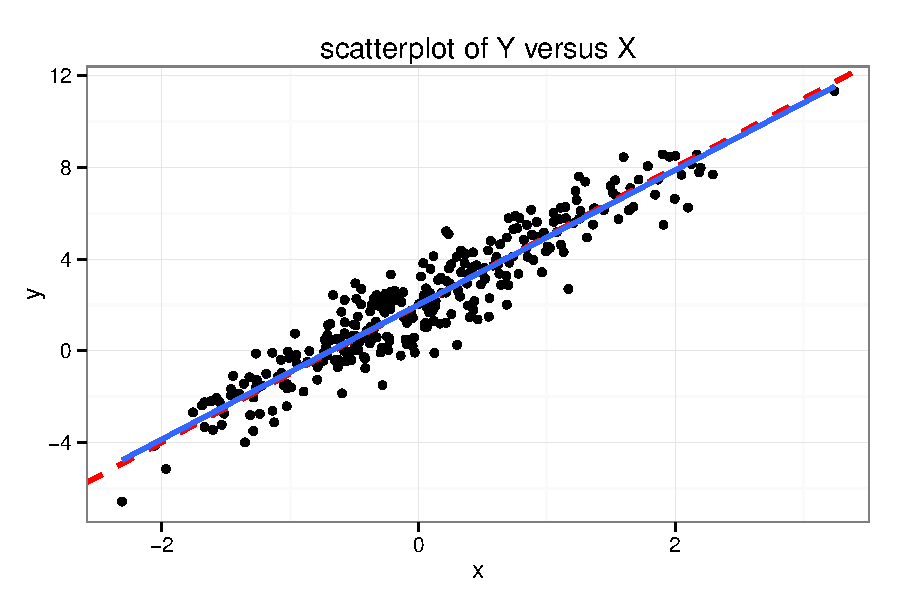
\includegraphics[width=.8\linewidth]{figure/p4121} 

}



\end{knitrout}

It's easy to see that the scatter of points is approximately elliptical. The solid line is the true regression line, the same as major axis of the ellipse, and the dashed line is the fitted regression line. Note that the fitted regression line is similar to, but not exactly the same as, the major axis of the ellipse.

\subproblem{4.12.2}
Repeat Problem 4.12.1 twice, first set $\sigma = 3$ and then repeat again with $\sigma = 6$. How does the scatter of points change as $\sigma$ changes?

\solution
\begin{knitrout}
\definecolor{shadecolor}{rgb}{1, 1, 1}\color{fgcolor}\begin{kframe}
\begin{alltt}
\hlstd{p1} \hlkwb{<-} \hlkwd{f412}\hlstd{(x,} \hlkwc{y} \hlstd{=} \hlnum{2} \hlopt{+} \hlnum{3} \hlopt{*} \hlstd{x} \hlopt{+} \hlkwd{rnorm}\hlstd{(}\hlkwc{n} \hlstd{= n,} \hlkwc{sd} \hlstd{=} \hlnum{3}\hlstd{))}
\hlstd{p1} \hlkwb{<-} \hlstd{p1} \hlopt{+} \hlkwd{ggtitle}\hlstd{(}\hlstr{"sigma = 3"}\hlstd{)} \hlopt{+} \hlkwd{theme}\hlstd{(}\hlkwc{text} \hlstd{=} \hlkwd{element_text}\hlstd{(}\hlkwc{size} \hlstd{=} \hlnum{14}\hlstd{))}
\hlstd{p2} \hlkwb{<-} \hlkwd{f412}\hlstd{(x,} \hlkwc{y} \hlstd{=} \hlnum{2} \hlopt{+} \hlnum{3} \hlopt{*} \hlstd{x} \hlopt{+} \hlkwd{rnorm}\hlstd{(}\hlkwc{n} \hlstd{= n,} \hlkwc{sd} \hlstd{=} \hlnum{6}\hlstd{))}
\hlstd{p2} \hlkwb{<-} \hlstd{p2} \hlopt{+} \hlkwd{ggtitle}\hlstd{(}\hlstr{"sigma = 6"}\hlstd{)} \hlopt{+} \hlkwd{theme}\hlstd{(}\hlkwc{text} \hlstd{=} \hlkwd{element_text}\hlstd{(}\hlkwc{size} \hlstd{=} \hlnum{14}\hlstd{))}
\hlkwd{grid.arrange}\hlstd{(p1, p2,} \hlkwc{ncol} \hlstd{=} \hlnum{2}\hlstd{)}
\end{alltt}
\end{kframe}

{\centering 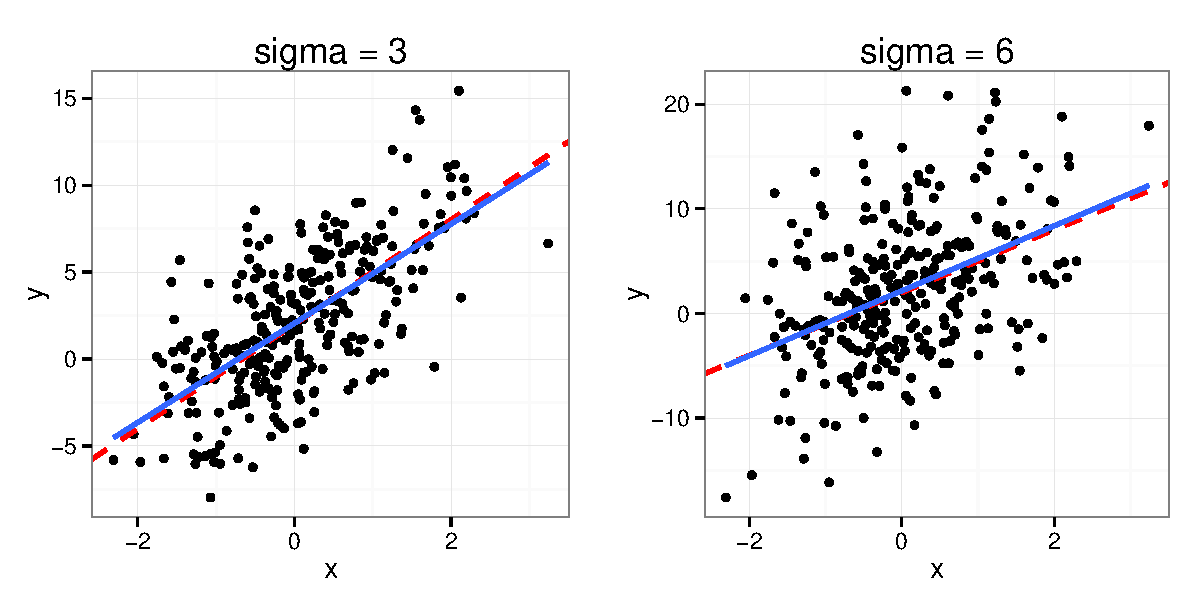
\includegraphics[width=.9\linewidth]{figure/p4122} 

}



\end{knitrout}

As the $\sigma$ increase, the conditional variance of y given x also increase.

\subproblem{4.12.3}
Repeat Problem 4.12.1, but this time set $X$ to have a standard normal distribution and $e$ to have a Cauchy distribution (set $\sigma = 1$). The easy way to generate a Cauchy is to generate two vectors $V_{1}$ and $V_{2}$ of standard normal random numbers, and then set $e = V_{1}/V_{2}$. With this setup, the values you generate are not bivariate normal because the Cauchy does not have a population mean or variance.

\solution
\begin{knitrout}
\definecolor{shadecolor}{rgb}{1, 1, 1}\color{fgcolor}\begin{kframe}
\begin{alltt}
\hlstd{e} \hlkwb{<-} \hlkwd{rnorm}\hlstd{(}\hlkwc{n} \hlstd{= n,} \hlkwc{sd} \hlstd{=} \hlnum{1}\hlstd{)} \hlopt{/} \hlkwd{rnorm}\hlstd{(}\hlkwc{n} \hlstd{= n,} \hlkwc{sd} \hlstd{=} \hlnum{1}\hlstd{)}
\hlstd{p3} \hlkwb{<-} \hlkwd{f412}\hlstd{(x,} \hlkwc{y} \hlstd{=} \hlnum{2} \hlopt{+} \hlnum{3} \hlopt{*} \hlstd{x} \hlopt{+} \hlstd{e)}
\hlstd{p3} \hlkwb{<-} \hlstd{p3} \hlopt{+} \hlkwd{ggtitle}\hlstd{(}\hlstr{"Cauchy Error"}\hlstd{)} \hlopt{+} \hlkwd{theme}\hlstd{(}\hlkwc{text} \hlstd{=} \hlkwd{element_text}\hlstd{(}\hlkwc{size} \hlstd{=} \hlnum{12}\hlstd{))}
\hlstd{p3}
\end{alltt}
\end{kframe}

{\centering 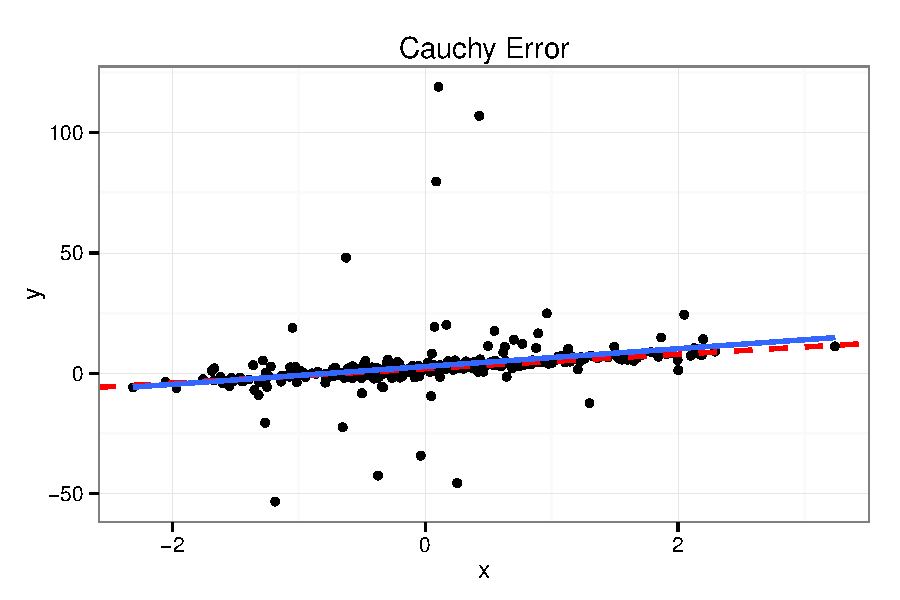
\includegraphics[width=.8\linewidth]{figure/p4123} 

}



\end{knitrout}

It seems that the scatter of points is not as elliptical as plot with normal error, and there exits many of extreme outliers.

\problem{5.8}
\textbf{Cake data} (Data file: \m{cakes})

\subproblem{5.8.1}
Fit (5.12) and verify that the significance levels for the quadratic terms and the interaction are all less than 0.005. When fitting polynomials, tests concerning main effects in models that include a quadratic are generally not of much interest.

\solution
\begin{knitrout}
\definecolor{shadecolor}{rgb}{1, 1, 1}\color{fgcolor}\begin{kframe}
\begin{alltt}
\hlstd{m} \hlkwb{<-} \hlkwd{lm}\hlstd{(Y} \hlopt{~} \hlstd{X1} \hlopt{+} \hlstd{X2} \hlopt{+} \hlkwd{I}\hlstd{(X1}\hlopt{^}\hlnum{2}\hlstd{)} \hlopt{+} \hlkwd{I}\hlstd{(X2}\hlopt{^}\hlnum{2}\hlstd{)} \hlopt{+} \hlkwd{I}\hlstd{(X1}\hlopt{*}\hlstd{X2),} \hlkwc{data} \hlstd{= cakes)}
\hlkwd{summary}\hlstd{(m)}
\end{alltt}
\begin{verbatim}
## 
## Call:
## lm(formula = Y ~ X1 + X2 + I(X1^2) + I(X2^2) + I(X1 * X2), data = cakes)
## 
## Residuals:
##    Min     1Q Median     3Q    Max 
## -0.491 -0.308  0.020  0.266  0.545 
## 
## Coefficients:
##              Estimate Std. Error t value Pr(>|t|)    
## (Intercept) -2.20e+03   2.42e+02   -9.13  1.7e-05 ***
## X1           2.59e+01   4.66e+00    5.56  0.00053 ***
## X2           9.92e+00   1.17e+00    8.50  2.8e-05 ***
## I(X1^2)     -1.57e-01   3.94e-02   -3.98  0.00408 ** 
## I(X2^2)     -1.20e-02   1.58e-03   -7.57  6.5e-05 ***
## I(X1 * X2)  -4.16e-02   1.07e-02   -3.88  0.00465 ** 
## ---
## Signif. codes:  0 '***' 0.001 '**' 0.01 '*' 0.05 '.' 0.1 ' ' 1
## 
## Residual standard error: 0.429 on 8 degrees of freedom
## Multiple R-squared:  0.949,	Adjusted R-squared:  0.917 
## F-statistic: 29.6 on 5 and 8 DF,  p-value: 5.86e-05
\end{verbatim}
\end{kframe}
\end{knitrout}

Note that the significance levels (p-value) for the quadratic terms and the interaction are all less than 0.005.

\subproblem{5.8.2}
The cake experiment was carried out in two blocks of seven observations each. It is possible that the response might differ by block. For example, if the blocks were different days, then differences in air temperature or humidity when the cakes were mixed might have some effect on $Y$. We can allow for block effects by adding a factor for block to the mean function and possibly allowing for block by regressor interactions. Add block effects to the mean function fit in Section 5.3.1 and summarize results. The blocking is indicated by the variable \m{Block} in the data file.

\solution
\begin{knitrout}
\definecolor{shadecolor}{rgb}{1, 1, 1}\color{fgcolor}\begin{kframe}
\begin{alltt}
\hlstd{cakes}\hlopt{$}\hlstd{block} \hlkwb{<-} \hlkwd{as.numeric}\hlstd{(}\hlkwd{as.character}\hlstd{(cakes}\hlopt{$}\hlstd{block))}
\hlstd{m1} \hlkwb{<-} \hlkwd{lm}\hlstd{(Y} \hlopt{~} \hlstd{X1} \hlopt{+} \hlstd{X2} \hlopt{+} \hlkwd{I}\hlstd{(X1}\hlopt{^}\hlnum{2}\hlstd{)} \hlopt{+} \hlkwd{I}\hlstd{(X2}\hlopt{^}\hlnum{2}\hlstd{)} \hlopt{+} \hlkwd{I}\hlstd{(X1}\hlopt{*}\hlstd{X2)} \hlopt{+}
             \hlstd{block} \hlopt{+} \hlkwd{I}\hlstd{(X1} \hlopt{*} \hlstd{block)} \hlopt{+} \hlkwd{I}\hlstd{(X2} \hlopt{*} \hlstd{block)} \hlopt{+}
             \hlkwd{I}\hlstd{(X1}\hlopt{^}\hlnum{2} \hlopt{*} \hlstd{block)} \hlopt{+} \hlkwd{I}\hlstd{(X2}\hlopt{^}\hlnum{2} \hlopt{*} \hlstd{block)} \hlopt{+}
             \hlkwd{I}\hlstd{(X1}\hlopt{*}\hlstd{X2} \hlopt{*} \hlstd{block),} \hlkwc{data} \hlstd{= cakes)}
\hlstd{m2} \hlkwb{<-} \hlkwd{step}\hlstd{(}\hlkwc{object} \hlstd{= m1,} \hlkwc{direction} \hlstd{=} \hlstr{"both"}\hlstd{,} \hlkwc{trace} \hlstd{=} \hlnum{FALSE}\hlstd{)}
\hlkwd{summary}\hlstd{(m2)}
\end{alltt}
\begin{verbatim}
## 
## Call:
## lm(formula = Y ~ X1 + X2 + I(X1^2) + I(X2^2) + I(X1 * X2) + I(X2 * 
##     block) + I(X1^2 * block), data = cakes)
## 
## Residuals:
##     Min      1Q  Median      3Q     Max 
## -0.3883 -0.0159  0.0001  0.0159  0.3417 
## 
## Coefficients:
##                  Estimate Std. Error t value Pr(>|t|)    
## (Intercept)     -2.20e+03   1.60e+02  -13.78  9.1e-06 ***
## X1               2.60e+01   3.08e+00    8.45  0.00015 ***
## X2               9.89e+00   7.71e-01   12.83  1.4e-05 ***
## I(X1^2)         -1.60e-01   2.61e-02   -6.15  0.00085 ***
## I(X2^2)         -1.19e-02   1.04e-03  -11.41  2.7e-05 ***
## I(X1 * X2)      -4.16e-02   7.08e-03   -5.88  0.00108 ** 
## I(X2 * block)   -1.64e-02   4.88e-03   -3.35  0.01536 *  
## I(X1^2 * block)  4.76e-03   1.39e-03    3.43  0.01394 *  
## ---
## Signif. codes:  0 '***' 0.001 '**' 0.01 '*' 0.05 '.' 0.1 ' ' 1
## 
## Residual standard error: 0.283 on 6 degrees of freedom
## Multiple R-squared:  0.983,	Adjusted R-squared:  0.964 
## F-statistic: 50.2 on 7 and 6 DF,  p-value: 6.63e-05
\end{verbatim}
\end{kframe}
\end{knitrout}

In this problem we fit regression model with regressors in problem 5.8.2, the main effect of \m{block} and interaction terms between \m{block} and all other predictors. We apply stepwise algorithm in this regression model to make sure that all effects contained in this model are of highly significance.

Note that the main effect of \m{block} is negligible, given other variable fixed. However, the interaction effect of \m{block} and \m{X2}, and \m{block} and $\m{X1}^2$ are significant, suggesting that the influence of \m{block} over the response is indirect.

\problem{5.14}
(Data file: \m{BGSall}) Refer to the Berkeley Guidance study described in Problem 3.3. Using the data file \m{BGSall}, consider the regression of \m{HT18} on \m{HT9} and the grouping factor \m{Sex}.

\subproblem{5.14.1}
Draw the scatterplot of \m{HT18} versus \m{HT9}, using a different symbol for males and females. Comment on the information in the graph about an appropriate mean function for these data.

\solution

\begin{knitrout}
\definecolor{shadecolor}{rgb}{1, 1, 1}\color{fgcolor}\begin{kframe}
\begin{alltt}
\hlstd{BGSall}\hlopt{$}\hlstd{Sex} \hlkwb{<-} \hlkwd{factor}\hlstd{(BGSall}\hlopt{$}\hlstd{Sex)}
\hlstd{p} \hlkwb{<-} \hlkwd{ggplot}\hlstd{(}\hlkwc{data} \hlstd{= BGSall,} \hlkwd{aes}\hlstd{(}\hlkwc{x} \hlstd{= HT9,} \hlkwc{y} \hlstd{= HT18))}
\hlstd{p} \hlkwb{<-} \hlstd{p} \hlopt{+} \hlkwd{geom_point}\hlstd{(}\hlkwd{aes}\hlstd{(}\hlkwc{shape} \hlstd{= Sex))}
\hlstd{p} \hlkwb{<-} \hlstd{p} \hlopt{+} \hlkwd{theme_bw}\hlstd{()} \hlopt{+} \hlkwd{theme}\hlstd{(}\hlkwc{text} \hlstd{=} \hlkwd{element_text}\hlstd{(}\hlkwc{size} \hlstd{=} \hlnum{12}\hlstd{))}
\hlstd{p} \hlkwb{<-} \hlstd{p} \hlopt{+} \hlkwd{geom_smooth}\hlstd{(}\hlkwc{formula} \hlstd{= y} \hlopt{~} \hlstd{x,} \hlkwc{method} \hlstd{=} \hlstr{"lm"}\hlstd{,} \hlkwc{se} \hlstd{=} \hlnum{FALSE}\hlstd{,} \hlkwc{size} \hlstd{=} \hlnum{1}\hlstd{,} \hlkwd{aes}\hlstd{(}\hlkwc{colour} \hlstd{= Sex))}
\hlstd{p} \hlkwb{<-} \hlstd{p} \hlopt{+} \hlkwd{ggtitle}\hlstd{(}\hlstr{"Scatterplot for Different Sex"}\hlstd{)}
\hlstd{p}
\end{alltt}
\end{kframe}

{\centering 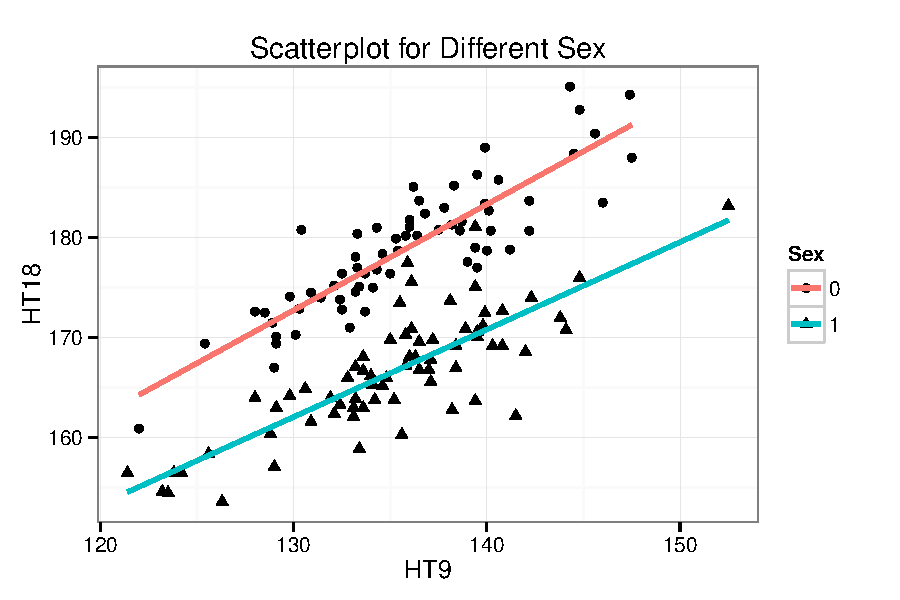
\includegraphics[width=.8\linewidth]{figure/p5141} 

}



\end{knitrout}

Note that the two slope coefficients of two mean functions are almost the same, but the intercepts are different, suggesting that given the same \m{HT9}, there exists significant difference of \m{HT18} for two levels of \m{Sex}.

\subproblem{5.14.2}
Obtain the appropriate test for a parallel regression model.

\solution

\begin{knitrout}
\definecolor{shadecolor}{rgb}{1, 1, 1}\color{fgcolor}\begin{kframe}
\begin{alltt}
\hlstd{m} \hlkwb{<-} \hlkwd{lm}\hlstd{(HT18} \hlopt{~} \hlstd{HT9} \hlopt{+} \hlstd{Sex,} \hlkwc{data} \hlstd{= BGSall)}
\hlkwd{summary}\hlstd{(m)}
\end{alltt}
\begin{verbatim}
## 
## Call:
## lm(formula = HT18 ~ HT9 + Sex, data = BGSall)
## 
## Residuals:
##     Min      1Q  Median      3Q     Max 
## -10.469  -2.095  -0.014   1.710  10.447 
## 
## Coefficients:
##             Estimate Std. Error t value Pr(>|t|)    
## (Intercept)  48.5173     7.3339    6.62  8.3e-10 ***
## HT9           0.9601     0.0539   17.82  < 2e-16 ***
## Sex1        -11.6958     0.5904  -19.81  < 2e-16 ***
## ---
## Signif. codes:  0 '***' 0.001 '**' 0.01 '*' 0.05 '.' 0.1 ' ' 1
## 
## Residual standard error: 3.43 on 133 degrees of freedom
## Multiple R-squared:  0.852,	Adjusted R-squared:  0.849 
## F-statistic:  382 on 2 and 133 DF,  p-value: <2e-16
\end{verbatim}
\end{kframe}
\end{knitrout}

We can add the group factor \m{Sex} into the original regression model, and see the t-test result of the coefficient of \m{Sex}. As the result, we see that the significance level of \m{Sex} is very low, suggesting that it should be a parallel regression model.

\subproblem{5.14.3}
Assuming the parallel regression model is adequate, estimate a 95\% confidence interval for the difference between males and females. For the parallel regression model, this is the difference in the intercepts of the two groups.

\solution
\begin{knitrout}
\definecolor{shadecolor}{rgb}{1, 1, 1}\color{fgcolor}\begin{kframe}
\begin{alltt}
\hlkwd{confint}\hlstd{(}\hlkwc{object} \hlstd{= m,} \hlkwc{level} \hlstd{=} \hlnum{.95}\hlstd{)}
\end{alltt}
\begin{verbatim}
##                2.5 %  97.5 %
## (Intercept)  34.0112  63.023
## HT9           0.8535   1.067
## Sex1        -12.8635 -10.528
\end{verbatim}
\end{kframe}
\end{knitrout}

To estimate a 95\% confidence interval for the difference between males and females, we only need obtain the 95\% confidence interval for the coefficient of \m{Sex}. As we can see, the confidence interval is $[-12.8635,~ -10.528$]
\end{document}


